\subsection{Image and video processing}
Because of the initial naïve designs, it was determined that image or video processing would be needed to be researched for finding the position of different elements. In this section, methods for detecting objects in an image are therefore being researched. It is necessary to figure out how to detect certain objects in the scene, to use it for controlling things in games or other interactive media.

\subsubsection{Color detection}
A very simple and useful way of detecting objects in a scene, is by using color detection. The drawbacks of this are that it is sometimes necessary to put certain colors on objects that will be used in the scene, in order to make them easier to detect. It is also a good idea to have a background with very few colors, so the colors are easier to separate. It can limit the colors the user can wear, for example if the camera is set to detect green colors and the user is wearing a green shirt. For example, if an image is searched for green colors, and the user is wearing green, the program will probably detect the user's shirt. While this might be exactly what the program should do, it would be beneficial to be able to control what to detect, and thus, eliminating uncontrollable elements.

Thresholding can be used to enable color detection. Thresholding is isolation of a color or a spectrum of colors. For example, to isolate objects that are very red, the statement r > 200 could be used(e.g. in C++). This would isolate all colors with a red value greater than 200, turning them white in the output image. Here is a simple example on how to use thresholding, written in pseudo-code. This is assuming the input is an RGB (red, green, and blue values) image, and the output is a grayscale image.

\begin{algorithm}[H]
\caption{Color thresholding}
\label{code:threshold}
\begin{algorithmic}
\IF {$ R>R_{min} \; and \; R<R_{max} \; and $\\
	 $ G>G_{min} \; and \; G<G_{max} \; and $\\
	 $ B>B_{min} \; and \; B<B_{max}$\\}
\STATE $g(x,y)=255$
\ELSE
\STATE $g(x,y = 0$
\ENDIF
\end{algorithmic}
\end{algorithm}

In the above example, g(x, y) is the output image, where the x and y is the position of the pixel current being processed. For most computers and image acquisition, the RGB color space is used, hence the lack of detail about how to use any other color spaces. In the Gesture Recognition chapter, other color spaces will be discussed, as they make more sense in that situation. The output of the above code would be a binary image. For each pixel in a binary image, it can only have two different values: 0 or 255. This ensures that it is easier for the program to work with, as it only have to compare two values, not 256 values.

Isolating a certain color is not enough to actually do something with it though. If one wishes to figure out what position a colored object is at, it is a good idea to find the average center of the detected color. A way of doing this is by finding the average position of all the white pixels in the output image. So, for each white pixel, assign its x and y position to one variable each, and have another variable that counts how many white pixels there are. Then, divide all the x values added together with the number of pixels, and do the same for all the y values.

The computer now knows the average position of a certain color in the scene. But what if the program should detect more colors? One way of doing this, is to avoid using a binary image for the output, and instead have the output be of many different values and or colors. Each thresholded color then has their own color in the output.

\subsubsection{BLOB analysis} \label{sec:blob}
BLOB stands for Binary Large OBject, and in image processing it represents a group of white or black pixels. As mentioned above, it is possible to detect several colors by having several colors in the output as well. This however means that the program cannot separate several objects of the same color. To fix this, a BLOB analysis could be used. To separate each BLOB, a so-called grassfire algorithm 
\footnote{A grassfire algorithm is an algorithm that detects and separates all BLOBs in a scene, by finding a detected pixel, and then labeling all connected pixels as one BLOB (also known as “burning” the pixels).} 
is usually used, with either 4- or 8-connectivity \parencite{Moeslund2012}. 4-connectivity checks the pixels above, below, to the left and to the right of the current pixel, whereas 8-connectivity also checks the pixels diagonally from the current pixel. 8-connectivity is more precise, since it is able to detect small diagonal lines unlike 4-connectivity, but it takes more processing power.
\bigskip

The recursive grassfire algorithm, “burns” every white pixel in an image, where the white pixels represent something that has been detected. It is called a recursive function, since it references itself. When the program searches through the image and encounters a white pixel, it will run a function containing the grassfire algorithm. This algorithm changes the white pixel to a gray pixel, with a value of 1-254. By doing this, the pixel is labelled with a number from 1-254, so the program can find these labelled pixels later. The reason we cannot use numbers below 1, is because that would label the pixel as being black, which the program ignores, and it cannot be labelled above 254, because the program detects it as something white which is has to make computations on, creating an infinite loop.

After labelling, the function will check if there is another white pixel next to the one it just marked. If there is, it will label that pixel with the same label as the one before (it will “burn” the pixel), and check if there are any white pixels next to that one. This continues until the function cannot find any more white pixels connected.
By doing this the program labels each white “island” of pixels, so it is easier to separate them and analyze each BLOB alone.

Note that there is also a sequential grassfire algorithm, which in some cases is more safe to use than the recursive one, since it does not risk running out of memory in the same way as the recursive. The computer only has a limited amount of memory allocated for function calls, and since the recursive function calls itself multiple times, it risks running out of memory if it encounters a very large BLOB, whereas the sequential algorithm does not call itself, and as such does not risk running out of memory. \parencite{Moeslund2012}

\subsubsection{Background Subtraction} \label{sec:BGSub}
The theory behind detecting changes in video is to have a reference image, and subtract that from the recorded image. This effectively removes the background in the image, and leaves only whatever change has been made in the picture. It is necessary to perform thresholding, and filter any noise away.

\subsubsection{Recognizing patterns} \label{sec:detect}
There exists several ways of detecting something in an image or a video feed, e.g. it might be necessary to detect how much something is rotated, which in turn could require template matching or other methods to find a certain object with a certain pattern. 
ARTag \parencite{Fiala2005}, a system built on such principles, uses a feature called a “fiducial marker”, which is an object that is placed in the view of the camera giving the possibility of detecting its position through visual computing.
\bigskip

\begin{figure}[!htbp]
\centering
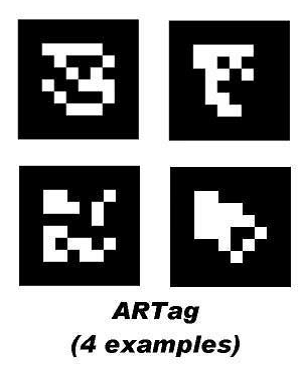
\includegraphics[scale=.5]{Artag}
\caption{Sample fiducial markers utilized in the software of ARTtag. \parencite{Fiala2005}}
\label{fig:artag}
\end{figure}

The fiducial markers used in the ARTag software are small patterns consisting of black and white squares (illustrated in figure \ref{fig:artag}).
One of the benefits for using these kinds of fiducial markers is the immunity to lighting conditions, i.e. variations in the lighting in the scene has a minimal effect on the detection. This is because of the patterns only being bitonal (in figure \ref{fig:artag} black and white only) and therefore reduces the decision made about each pixel to a threshold decision. 
Furthermore, with the technology of ARTag, the rate of detecting an object, or a pattern, when it does not exist in the scene is reduced to just 0.0039\% (1/26,000).
Seen in contrast to basic color detection, where the background partially could consist of the same color as the object being detected, ARTag takes very good care of this issue. The downside of such a system, compared to a basic color detection system, is that the system requires more processing power.


\subsubsection{Summary}
Color detection is achieved by using thresholding, which isolates certain colors so they can be detected. Color detection is useful if the program only needs to detect one color, or if it needs to detect more than one easily detectable color (for example detection of red, green and blue, in an otherwise white scene).

However if for example a program is required to detect two different players in a two player game, where each player is holding up a red sticker for detection, the program needs to separate these two colors. This is where BLOB detection comes in use, by detecting each BLOB of white pixels, by using a grassfire algorithm. Note that BLOB detection can be used in turn with almost any other detection method, in order to separate objects in the scene.

If the program needs to detect objects that enter a scene, the program can have a reference image of the scene without any objects, and then subtract that image from the video feed. Anything that enters will then stand out. \parencite{Moeslund2012}
